\section{Correlated bivariate distribution}

\begin{tcolorbox}[width=\linewidth, sharp corners=all, colback=white!95!black]
Let $(X,Y)$ follow a bivariate normal standard distribution with correlation $\rho$. Find the expectation: $$\mathbb{E}[\operatorname{sgn}(X)\operatorname{sgn}(Y)].$$
\end{tcolorbox}

$$(X,Y) \sim \mathcal{N}\left(\begin{pmatrix}0\\0\end{pmatrix}, \begin{pmatrix}
1 & \rho\\ \rho & 1
\end{pmatrix}\right).$$

To see what happens here, we can compare the density contour of this distribution with the independent case. The covariance matrix is symmetric thus diagonalizable. We can find its eigenvalues and its eigenvectors (through classic computations or noticing this is a circulant matrix). With $P = \begin{pmatrix}
1 & 1\\ 1 & -1
\end{pmatrix}$,
$$\Sigma = P\begin{pmatrix}
1+\rho & 0\\ 0 & 1-\rho
\end{pmatrix}P^{-1}.$$
This gives us the shape of the correlated distribution. Qualitatively, we can say that, as $\rho$ defines how rotated and squished the distribution is, the bigger $\rho$, the higher the probabiliy of $X$ and $Y$ being the same sign.

\begin{figure}[H]
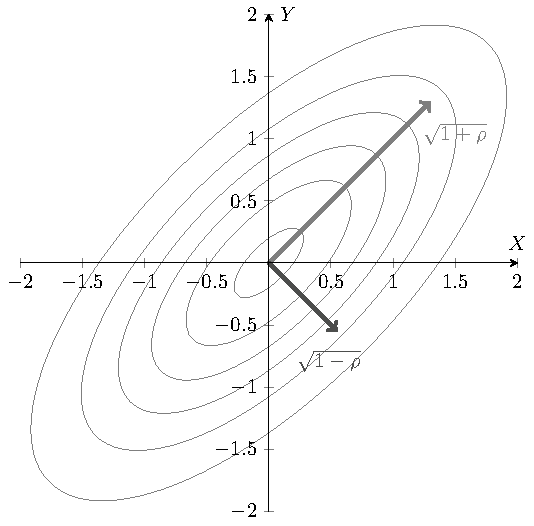
\includegraphics[width=0.35\textwidth]{img/tikz/bivariate_contour.pdf}
\centering
\caption{Density contours of a bivariate normal law, with $\rho=0.7$}
\label{fig:bivariate_contour}
\end{figure}


Back to our problem: the random variable $\operatorname{sgn}(X)\operatorname{sgn}(Y)$ takes values in the set $\{-1,1\}$. Thus, to get its expectancy, we can compute these discrete probabilities :
\begin{align*}
    \mathbb{E}[\operatorname{sgn}(X)\operatorname{sgn}(Y)] &= 1\times \mathbb{P}(\operatorname{sgn}(X)\operatorname{sgn}(Y)=1) -1\times \mathbb{P}(\operatorname{sgn}(X)\operatorname{sgn}(Y)=-1)\\
    &= 1\times \mathbb{P}(\operatorname{sgn}(X)\operatorname{sgn}(Y)=1) -1\times (1-\mathbb{P}(\operatorname{sgn}(X)\operatorname{sgn}(Y)=1))\\
    &= 2\mathbb{P}(\operatorname{sgn}(X)\operatorname{sgn}(Y)=1) -1.
\end{align*}

Using the symmetry of the distribution, $$\mathbb{P}(\operatorname{sgn}(X)\operatorname{sgn}(Y)=1) = \mathbb{P}(X>0,Y>0) + \mathbb{P}(X<0,Y<0) = 2\mathbb{P}(X>0,Y>0),$$

thus the only thing we need to compute is $\mathbb{P}(X>0,Y>0)$.\\

If $$\begin{pmatrix}U\\V\end{pmatrix} = \Sigma^{-1/2}\begin{pmatrix}X\\Y\end{pmatrix},$$
then $(U,V)$ follows an independent bivariate normal standard distribution. Inverting $\Sigma$ we get:
$$\Sigma^{-1} = \frac1{1-\rho^2}\begin{pmatrix}
1 & -\rho\\ -\rho & 1
\end{pmatrix}.$$

\begin{figure}[H]
    \centering
    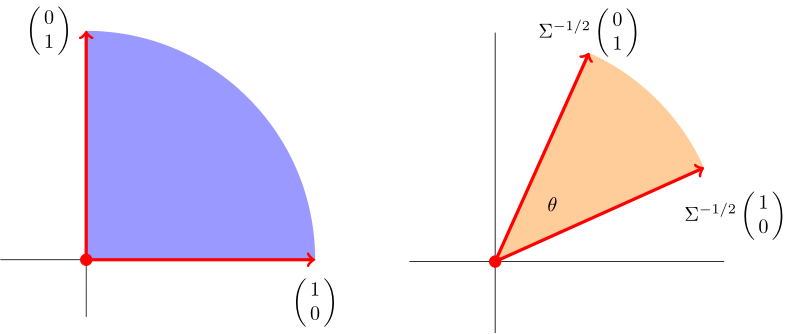
\includegraphics[width=0.8\textwidth]{img/corr_biv_normal.png}
    \caption{Area of the event $X>0,Y>0$ for $\rho = 0$ (left) and $\rho \ne 0$ (right). From \href{https://math.stackexchange.com/questions/1687795/correlated-joint-normal-distribution-calculating-a-probability}{here}.}
\end{figure}

Then, there exists a $\theta \in [0,2\pi]$ such that $\mathbb{P}(X>0,Y>0) = \dfrac{\theta}{2\pi}$. This $\theta$ verifies $$\cos{\theta} = \dfrac{\langle u,v\rangle}{\|u\| \|v\|}.$$ with $u = \Sigma^{-1/2} \begin{pmatrix}1\\0\end{pmatrix}$ and $v = \Sigma^{-1/2} \begin{pmatrix}0\\1\end{pmatrix}$


$$\langle u,v\rangle = (1\ 0)\,\Sigma^{-1}(0\ 1)^T=-\rho/(1-\rho^2)$$
$$\|u\|^2=(1\ 0)\,\Sigma^{-1}(1\ 0)^T=1/(1-\rho^2)$$
$$\|v\|^2=(0\ 1)\,\Sigma^{-1}(0\ 1)^T=1/(1-\rho^2)$$

so that $\cos(\theta)=-\rho.$ Putting it all together gives 
$$\mathbb{P}(X>0,Y>0)=\dfrac{\arccos(-\rho)}{ 2\pi}.$$

Finally, $$\boxed{ \mathbb{E}[\operatorname{sgn}(X)\operatorname{sgn}(Y)] = \dfrac{2\arccos(-\rho)}{\pi} - 1. }$$

Note that if $\rho=0$, we have $\mathbb{E}[\operatorname{sgn}(X)\operatorname{sgn}(Y)]=0$ ; it converges to $1$ as $\rho \longrightarrow 1$ and to $-1$ as $\rho \longrightarrow -1$, which gives us confidence in our answer.
